\documentclass{beamer}
\usetheme{Warsaw}
\setbeamertemplate{footline}[frame number]

\usepackage[utf8]{inputenc}
\usepackage{fancybox}
\usepackage{multimedia} 
\usepackage{subfig}
\usepackage{amsmath}
\usepackage{hyperref}
% Setze die Optionen für das hyperref-Paket
\hypersetup{
    colorlinks=true,    % Färbt die Links
    linkcolor=blue,     % Farbe für interne Links
    filecolor=magenta,  % Farbe für Links zu lokalen Dateien
    urlcolor=cyan,      % Farbe für externe Links
    pdftitle={Angewandte Mathematik}, % Titel des Dokuments
    pdfpagemode=FullScreen, % Öffnet das PDF im Vollbildmodus
}

\usepackage[all]{xy}
\begin{document}


\title[Angewandte Mathematik] % (optional, only for long titles)
{Angewandte Mathematik
\\
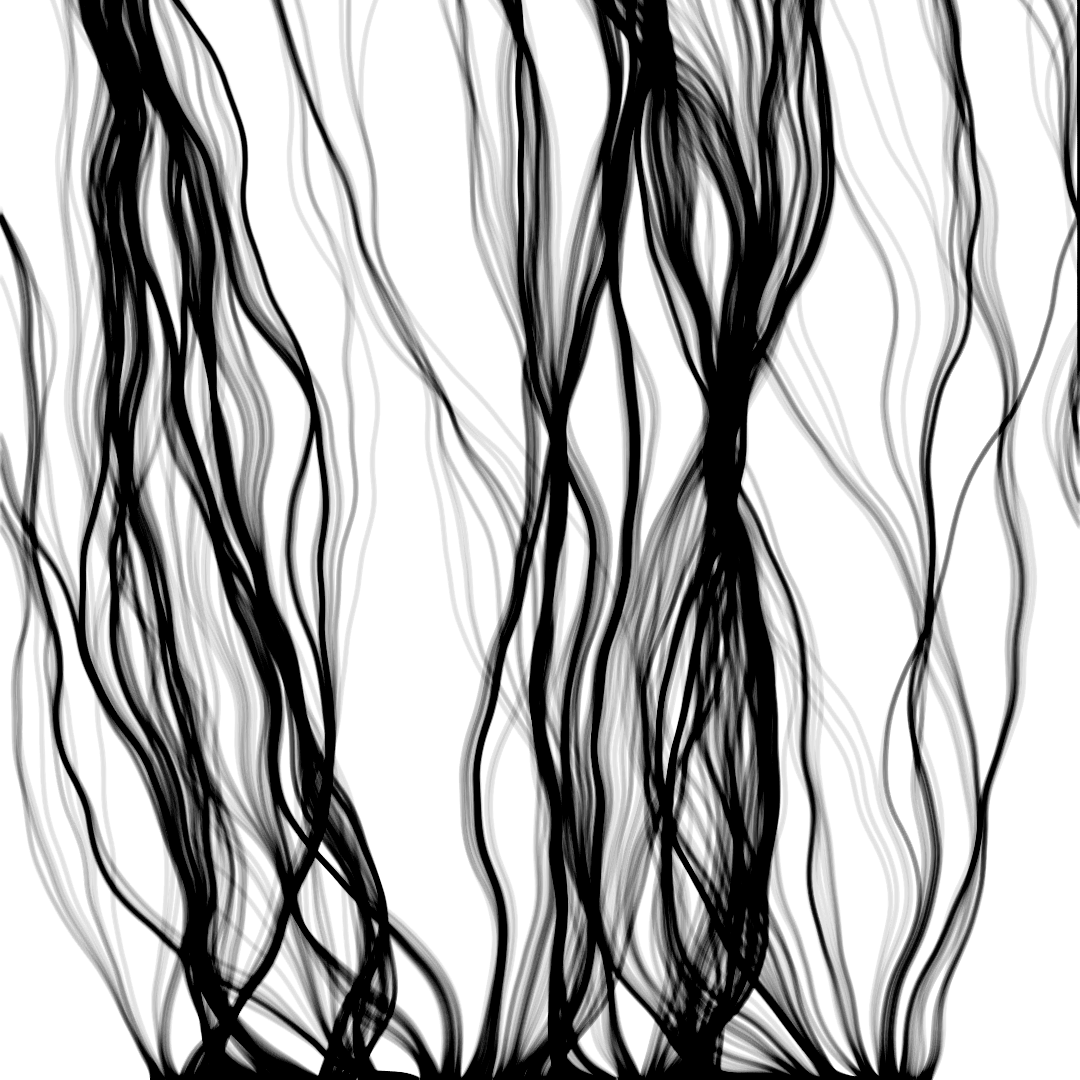
\includegraphics[scale=0.15]{images/cover}
}
\subtitle{}
\author[Dr. Johannes Riesterer] % (optional, for multiple authors)
{Dr.  rer. nat. Johannes Riesterer}

\date[KPT 2004] % (optional)
{}

\subject{Angewandte Mathematik}

\frame{\titlepage}

\begin{frame}
    \frametitle{Angewandte Mathematik}
    \framesubtitle{Asymptotics}
    \begin{block}{Für hinreichend groß \href{https://github.com/leanprover-community/mathlib4/blob/418a5eb7aec3fb639097cb13f74fc031ac4057f2/Mathlib/Order/Filter/Defs.lean\#L243-L244}{Mathlib}}
        Für einen Filter $l$ bedeutet die Bedingung 
        \( \forall^f x \;  p(x) \) 
       dass die Menge der Elemente, für die \( p(x) \) gilt, ein Element des Filters \( f \) ist, also
        \( \{ X \; | \;  p(x) \} \in l \).
    \end{block}
\end{frame}

\begin{frame}
    \frametitle{Angewandte Mathematik}
    \framesubtitle{Asymptotics}
    \begin{block}{Landau-O-Notation (Großes \( O \)) \href{https://github.com/leanprover-community/mathlib4/blob/418a5eb7aec3fb639097cb13f74fc031ac4057f2/Mathlib/Analysis/Asymptotics/Asymptotics.lean\#L75-L80}{Mathlib}
        }
        Für einen filter $l$ und funktionen $g,h$
    \( f(n) = O(g(n)) \) bedeutet, dass \( f(n) \) asymptotisch nach oben durch \( g(n) \) beschränkt ist. Das heißt, es existieren Konstanten \( C > 0 \) und \( n_0 \), sodass für alle \( n \geq n_0 \) gilt:
    \[
    |f(n)| \leq C \cdot |g(n)|.
    \]
    \end{block}

    \begin{exampleblock}{Beispiel} 
    Sei \( f(n) = 3n^2 + 2n + 1 \), dann gilt:
    \[
    f(n) = O(n^2),
    \]
    da für große \( n \) der \( n^2 \)-Term dominiert.
    \end{exampleblock}
\end{frame}

\begin{frame}
    \frametitle{Angewandte Mathematik}
    \framesubtitle{Asymptotics}
    
    \begin{block}{Landau-Klein-o-Notation (kleines \( o \))}
        \( f(n) = o(g(n)) \) bedeutet, dass \( f(n) \) im Vergleich zu \( g(n) \) asymptotisch vernachlässigbar ist. Für jede Konstante \( C > 0 \) existiert ein \( n_0 \), sodass für alle \( n \geq n_0 \) gilt:
        \[
        |f(n)| \leq C \cdot |g(n)|.
        \]
        Dies impliziert, dass \( f(n) \) wesentlich kleiner als \( g(n) \) wird, wenn \( n \to \infty \).
    \end{block}

    \begin{exampleblock}{Beispiel}
        Sei \( f(n) = n \) und \( g(n) = n^2 \), dann gilt:
        \[
        f(n) = o(n^2),
        \]
        da \( n \) wesentlich langsamer als \( n^2 \) wächst.
    \end{exampleblock}
\end{frame}

\begin{frame}
    \frametitle{Angewandte Mathematik}
    \framesubtitle{Asymptotics}
 
    \begin{block}{Implikationen zwischen \( O \)- und \( o \)-Notation}
        \begin{itemize}
            \item \( f(n) = o(g(n)) \) impliziert \( f(n) = O(g(n)) \), da \( o(g(n)) \) eine strengere Schranke als \( O(g(n)) \) ist.
            \item Umgekehrt gilt jedoch: \( f(n) = O(g(n)) \) impliziert nicht, dass \( f(n) = o(g(n)) \). Beispiel: \( f(n) = 2n \) und \( g(n) = n \) führen zu \( f(n) = O(n) \), aber \( f(n) \neq o(n) \).
        \end{itemize}
    \end{block}

    \begin{exampleblock}{Zusammenfassung}
        \[
        o(g(n)) \implies O(g(n)),
        \]
        aber nicht umgekehrt.
    \end{exampleblock}
\end{frame}

\end{document}
